% fig4c-basins.tex
\documentclass[tikz,border=5pt]{standalone}
% common-styles.tex
% Shared TikZ styles for wonton-proof paper figures

\usepackage{silence}
\WarningFilter{latex}{Missing character} 
\tracinglostchars=0 % Suppress engine-level "Missing character" warnings

\usepackage{fontspec}
\usepackage{unicode-math}

% Use filenames for reliability with Tectonic
\setmainfont{LibertinusSerif-Regular.otf}[
    BoldFont=LibertinusSerif-Bold.otf,
    ItalicFont=LibertinusSerif-Italic.otf,
    BoldItalicFont=LibertinusSerif-BoldItalic.otf
]
\setsansfont{LibertinusSans-Regular.otf}[
    BoldFont=LibertinusSans-Bold.otf,
    ItalicFont=LibertinusSans-Italic.otf
]
\setmonofont{LibertinusMono-Regular.otf}

% Try a more standard math font if LibertinusMath is causing nullfont issues
\setmathfont{LibertinusMath-Regular.otf}
% \setmathfont{latinmodern-math.otf}[range=digits] 

\usepackage{amsmath}
\usepackage{tikz}
\usepackage{forest}

\usetikzlibrary{
    arrows.meta,
    calc,
    decorations.pathreplacing,
    fit,
    positioning,
    shapes.geometric,
    shapes.misc,
    backgrounds,
    shadows.blur,
    fadings
}

% Color palette (muted, print-friendly)
\definecolor{ink}{RGB}{45,45,52}
\definecolor{muted}{RGB}{115,115,125}
\definecolor{highlight}{RGB}{198,120,44}
\definecolor{accentblue}{RGB}{86,130,178}
\definecolor{accentgreen}{RGB}{84,156,132}
\definecolor{blocked}{RGB}{140,75,75}
\definecolor{goalnode}{RGB}{255,255,255}
\definecolor{terminal}{RGB}{238,239,244}
\definecolor{deadnode}{RGB}{248,245,245}
\definecolor{flowbox}{RGB}{250,250,252}
\definecolor{basin1}{RGB}{224,234,248}
\definecolor{basin2}{RGB}{246,232,221}
\definecolor{basin3}{RGB}{228,242,234}
\definecolor{heatbase}{RGB}{86,130,178}

\tikzset{
    line cap=round,
    line join=round,
    pop/.style={
        blur shadow={shadow blur steps=5, shadow blur extra rounding=1.3pt}
    },
    base node/.style={
        rounded rectangle,
        draw=ink,
        line width=0.6pt,
        fill=goalnode,
        text=ink,
        minimum width=2.2cm,
        minimum height=0.7cm,
        align=center,
        pop
    },
    goal/.style={base node, fill=goalnode},
    terminal/.style={base node, fill=terminal, line width=0.9pt},
    dead/.style={base node, fill=deadnode, dashed},
    flowbox/.style={
        rectangle,
        draw=muted,
        rounded corners=3pt,
        fill=flowbox,
        minimum width=1.8cm,
        minimum height=0.6cm,
        align=center,
        font=\normalfont\small,
        text=ink,
        pop
    },
    decision/.style={
        diamond,
        draw=muted,
        fill=flowbox,
        aspect=2.4,
        font=\normalfont\small,
        inner sep=1pt,
        text=ink
    },
    protocolbox/.style={
        rectangle,
        draw=muted,
        rounded corners=4pt,
        fill=flowbox,
        minimum width=2cm,
        minimum height=0.8cm,
        font=\normalfont\small,
        align=center,
        text=ink
    },
    tactic/.style={
        ->,
        >=Stealth,
        draw=muted,
        line width=0.75pt
    },
    tacticlight/.style={
        ->,
        >=Stealth,
        draw=muted!45,
        dashed,
        line width=0.6pt
    },
    backprop/.style={
        ->,
        >=Stealth,
        draw=muted!70,
        dashed,
        line width=0.6pt
    },
    selected/.style={
        tactic,
        draw=highlight,
        line width=1.4pt
    },
    divergetactic/.style={
        tactic,
        draw=highlight,
        line width=1.4pt
    },
    divergenode/.style={
        base node,
        draw=highlight,
        line width=1.0pt
    },
    divergeblock/.style={
        blockedtactic,
        line width=1.2pt
    },
    blockedtactic/.style={
        tactic,
        draw=blocked,
        densely dashed
    },
    flowarrow/.style={
        ->,
        >=Stealth,
        draw=muted,
        line width=0.75pt
    },
    crosslink/.style={
        -,
        draw=muted!70,
        dotted,
        line width=0.6pt
    },
    annot/.style={
        font=\normalfont\footnotesize,
        text=muted
    },
    visit/.style={
        annot,
        font=\normalfont\scriptsize
    },
    annotbg/.style={
        annot,
        fill=white,
        inner sep=1.5pt
    },
    tacticlabel/.style={
        annot,
        font=\ttfamily\footnotesize,
        text=muted
    },
    formula/.style={
        font=\normalfont\footnotesize,
        draw=muted,
        rounded corners=2pt,
        fill=white,
        inner sep=3pt
    },
    paneltitle/.style={
        font=\normalfont\bfseries,
        text=ink
    },
    trajectory/.style={
        ->,
        draw=muted!70,
        line width=0.6pt
    }
}

\begin{document}
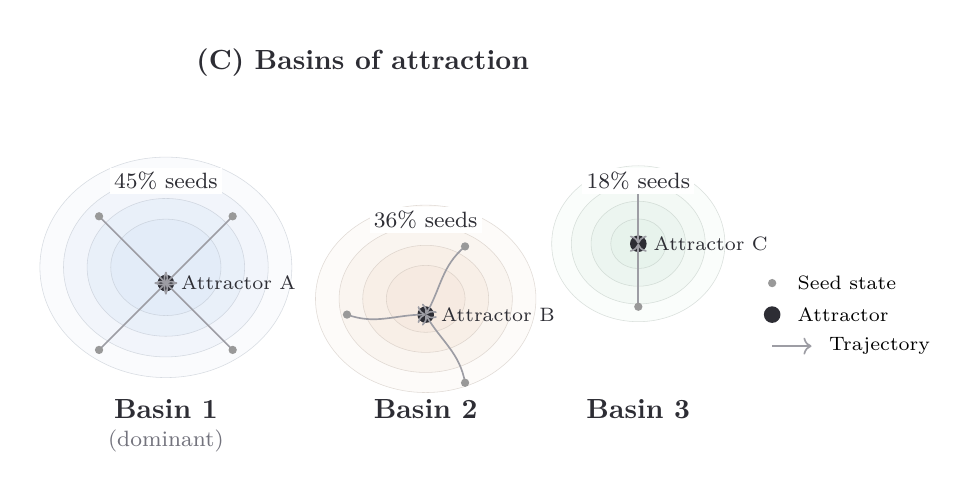
\begin{tikzpicture}[
    every node/.style={font=\small},
    show background rectangle,
    background rectangle/.style={fill=white}
]

\begin{scope}[shift={(0, 0)}]
    \node[paneltitle, anchor=south] at (4.0, 3.5) {(C) Basins of attraction};

    % Basin 1 (Topological Contours)
    \foreach \r/\o in {1.6/0.15, 1.3/0.3, 1.0/0.45, 0.7/0.6} {
        \pgfmathsetmacro{\ry}{\r*0.875}
        \fill[basin1, opacity=\o] (1.5, 1.2) ellipse (\r cm and \ry cm);
        \draw[basin1!80!black, line width=0.2pt, opacity=0.5] (1.5, 1.2) ellipse (\r cm and \ry cm);
    }
    \node[font=\bfseries, text=ink] at (1.5, -0.6) {Basin 1};
    \node[annot] at (1.5, -1.0) {(dominant)};
    \fill[ink] (1.5, 1.0) circle (3pt) node[right, xshift=2pt, font=\scriptsize] {Attractor A};

    % Basin 2 (Topological Contours)
    \foreach \r/\o in {1.4/0.15, 1.1/0.3, 0.8/0.45, 0.5/0.6} {
        \pgfmathsetmacro{\ry}{\r*0.85}
        \fill[basin2, opacity=\o] (4.8, 0.8) ellipse (\r cm and \ry cm);
        \draw[basin2!80!black, line width=0.2pt, opacity=0.5] (4.8, 0.8) ellipse (\r cm and \ry cm);
    }
    \node[font=\bfseries, text=ink] at (4.8, -0.6) {Basin 2};
    \fill[ink] (4.8, 0.6) circle (3pt) node[right, xshift=2pt, font=\scriptsize] {Attractor B};

    % Basin 3 (Topological Contours)
    \foreach \r/\o in {1.1/0.15, 0.85/0.3, 0.6/0.45, 0.35/0.6} {
        \pgfmathsetmacro{\ry}{\r*0.9}
        \fill[basin3, opacity=\o] (7.5, 1.5) ellipse (\r cm and \ry cm);
        \draw[basin3!80!black, line width=0.2pt, opacity=0.5] (7.5, 1.5) ellipse (\r cm and \ry cm);
    }
    \node[font=\bfseries, text=ink] at (7.5, -0.6) {Basin 3};
    \fill[ink] (7.5, 1.5) circle (3pt) node[right, xshift=2pt, font=\scriptsize] {Attractor C};

    % Trajectories
    % Basin 1 trajectories
    \foreach \ang in {45, 135, 225, 315} {
        \draw[trajectory, ->] ($(1.5, 1.0) + (\ang:1.2)$) to[out=\ang+180, in=\ang] (1.5, 1.0);
        \fill[black!40] ($(1.5, 1.0) + (\ang:1.2)$) circle (1.5pt);
    }
    % Basin 2 trajectories
    \foreach \ang in {60, 180, 300} {
         \draw[trajectory, ->] ($(4.8, 0.6) + (\ang:1.0)$) to[out=\ang+160, in=\ang] (4.8, 0.6);
         \fill[black!40] ($(4.8, 0.6) + (\ang:1.0)$) circle (1.5pt);
    }
    % Basin 3 trajectories
    \foreach \ang in {90, 270} {
         \draw[trajectory, ->] ($(7.5, 1.5) + (\ang:0.8)$) to[out=\ang+180, in=\ang] (7.5, 1.5);
         \fill[black!40] ($(7.5, 1.5) + (\ang:0.8)$) circle (1.5pt);
    }

    % Stats
    \node[annotbg, text=ink] at (1.5, 2.3) {45\% seeds};
    \node[annotbg, text=ink] at (4.8, 1.8) {36\% seeds};
    \node[annotbg, text=ink] at (7.5, 2.3) {18\% seeds};

    % Legend
    \begin{scope}[shift={(9.2, 1.0)}]
        \fill[black!40] (0, 0) circle (1.5pt);
        \node[anchor=west, font=\scriptsize] at (0.2, 0) {Seed state};

        \fill[ink] (0, -0.4) circle (3pt);
        \node[anchor=west, font=\scriptsize] at (0.2, -0.4) {Attractor};

        \draw[trajectory, ->] (0, -0.8) -- (0.5, -0.8);
        \node[anchor=west, font=\scriptsize] at (0.6, -0.8) {Trajectory};
    \end{scope}
\end{scope}
\end{tikzpicture}
\end{document}